% Options for packages loaded elsewhere
\PassOptionsToPackage{unicode}{hyperref}
\PassOptionsToPackage{hyphens}{url}
%
\documentclass[
]{article}
\usepackage{amsmath,amssymb}
\usepackage{lmodern}
\usepackage{iftex}
\ifPDFTeX
  \usepackage[T1]{fontenc}
  \usepackage[utf8]{inputenc}
  \usepackage{textcomp} % provide euro and other symbols
\else % if luatex or xetex
  \usepackage{unicode-math}
  \defaultfontfeatures{Scale=MatchLowercase}
  \defaultfontfeatures[\rmfamily]{Ligatures=TeX,Scale=1}
\fi
% Use upquote if available, for straight quotes in verbatim environments
\IfFileExists{upquote.sty}{\usepackage{upquote}}{}
\IfFileExists{microtype.sty}{% use microtype if available
  \usepackage[]{microtype}
  \UseMicrotypeSet[protrusion]{basicmath} % disable protrusion for tt fonts
}{}
\makeatletter
\@ifundefined{KOMAClassName}{% if non-KOMA class
  \IfFileExists{parskip.sty}{%
    \usepackage{parskip}
  }{% else
    \setlength{\parindent}{0pt}
    \setlength{\parskip}{6pt plus 2pt minus 1pt}}
}{% if KOMA class
  \KOMAoptions{parskip=half}}
\makeatother
\usepackage{xcolor}
\usepackage[margin=1in]{geometry}
\usepackage{color}
\usepackage{fancyvrb}
\newcommand{\VerbBar}{|}
\newcommand{\VERB}{\Verb[commandchars=\\\{\}]}
\DefineVerbatimEnvironment{Highlighting}{Verbatim}{commandchars=\\\{\}}
% Add ',fontsize=\small' for more characters per line
\usepackage{framed}
\definecolor{shadecolor}{RGB}{248,248,248}
\newenvironment{Shaded}{\begin{snugshade}}{\end{snugshade}}
\newcommand{\AlertTok}[1]{\textcolor[rgb]{0.94,0.16,0.16}{#1}}
\newcommand{\AnnotationTok}[1]{\textcolor[rgb]{0.56,0.35,0.01}{\textbf{\textit{#1}}}}
\newcommand{\AttributeTok}[1]{\textcolor[rgb]{0.77,0.63,0.00}{#1}}
\newcommand{\BaseNTok}[1]{\textcolor[rgb]{0.00,0.00,0.81}{#1}}
\newcommand{\BuiltInTok}[1]{#1}
\newcommand{\CharTok}[1]{\textcolor[rgb]{0.31,0.60,0.02}{#1}}
\newcommand{\CommentTok}[1]{\textcolor[rgb]{0.56,0.35,0.01}{\textit{#1}}}
\newcommand{\CommentVarTok}[1]{\textcolor[rgb]{0.56,0.35,0.01}{\textbf{\textit{#1}}}}
\newcommand{\ConstantTok}[1]{\textcolor[rgb]{0.00,0.00,0.00}{#1}}
\newcommand{\ControlFlowTok}[1]{\textcolor[rgb]{0.13,0.29,0.53}{\textbf{#1}}}
\newcommand{\DataTypeTok}[1]{\textcolor[rgb]{0.13,0.29,0.53}{#1}}
\newcommand{\DecValTok}[1]{\textcolor[rgb]{0.00,0.00,0.81}{#1}}
\newcommand{\DocumentationTok}[1]{\textcolor[rgb]{0.56,0.35,0.01}{\textbf{\textit{#1}}}}
\newcommand{\ErrorTok}[1]{\textcolor[rgb]{0.64,0.00,0.00}{\textbf{#1}}}
\newcommand{\ExtensionTok}[1]{#1}
\newcommand{\FloatTok}[1]{\textcolor[rgb]{0.00,0.00,0.81}{#1}}
\newcommand{\FunctionTok}[1]{\textcolor[rgb]{0.00,0.00,0.00}{#1}}
\newcommand{\ImportTok}[1]{#1}
\newcommand{\InformationTok}[1]{\textcolor[rgb]{0.56,0.35,0.01}{\textbf{\textit{#1}}}}
\newcommand{\KeywordTok}[1]{\textcolor[rgb]{0.13,0.29,0.53}{\textbf{#1}}}
\newcommand{\NormalTok}[1]{#1}
\newcommand{\OperatorTok}[1]{\textcolor[rgb]{0.81,0.36,0.00}{\textbf{#1}}}
\newcommand{\OtherTok}[1]{\textcolor[rgb]{0.56,0.35,0.01}{#1}}
\newcommand{\PreprocessorTok}[1]{\textcolor[rgb]{0.56,0.35,0.01}{\textit{#1}}}
\newcommand{\RegionMarkerTok}[1]{#1}
\newcommand{\SpecialCharTok}[1]{\textcolor[rgb]{0.00,0.00,0.00}{#1}}
\newcommand{\SpecialStringTok}[1]{\textcolor[rgb]{0.31,0.60,0.02}{#1}}
\newcommand{\StringTok}[1]{\textcolor[rgb]{0.31,0.60,0.02}{#1}}
\newcommand{\VariableTok}[1]{\textcolor[rgb]{0.00,0.00,0.00}{#1}}
\newcommand{\VerbatimStringTok}[1]{\textcolor[rgb]{0.31,0.60,0.02}{#1}}
\newcommand{\WarningTok}[1]{\textcolor[rgb]{0.56,0.35,0.01}{\textbf{\textit{#1}}}}
\usepackage{longtable,booktabs,array}
\usepackage{calc} % for calculating minipage widths
% Correct order of tables after \paragraph or \subparagraph
\usepackage{etoolbox}
\makeatletter
\patchcmd\longtable{\par}{\if@noskipsec\mbox{}\fi\par}{}{}
\makeatother
% Allow footnotes in longtable head/foot
\IfFileExists{footnotehyper.sty}{\usepackage{footnotehyper}}{\usepackage{footnote}}
\makesavenoteenv{longtable}
\usepackage{graphicx}
\makeatletter
\def\maxwidth{\ifdim\Gin@nat@width>\linewidth\linewidth\else\Gin@nat@width\fi}
\def\maxheight{\ifdim\Gin@nat@height>\textheight\textheight\else\Gin@nat@height\fi}
\makeatother
% Scale images if necessary, so that they will not overflow the page
% margins by default, and it is still possible to overwrite the defaults
% using explicit options in \includegraphics[width, height, ...]{}
\setkeys{Gin}{width=\maxwidth,height=\maxheight,keepaspectratio}
% Set default figure placement to htbp
\makeatletter
\def\fps@figure{htbp}
\makeatother
\setlength{\emergencystretch}{3em} % prevent overfull lines
\providecommand{\tightlist}{%
  \setlength{\itemsep}{0pt}\setlength{\parskip}{0pt}}
\setcounter{secnumdepth}{-\maxdimen} % remove section numbering
\ifLuaTeX
  \usepackage{selnolig}  % disable illegal ligatures
\fi
\IfFileExists{bookmark.sty}{\usepackage{bookmark}}{\usepackage{hyperref}}
\IfFileExists{xurl.sty}{\usepackage{xurl}}{} % add URL line breaks if available
\urlstyle{same} % disable monospaced font for URLs
\hypersetup{
  pdftitle={Verkefni1 - MAS201F},
  hidelinks,
  pdfcreator={LaTeX via pandoc}}

\title{Verkefni1 - MAS201F}
\author{}
\date{\vspace{-2.5em}2023-01-12}

\begin{document}
\maketitle

Monty Hall þrautin gengur út á það að einstaklingur á að ímynda sér að
hann sé að taka þátt í leik í sjónvarspsþætti og fái val um þrjár hurðir
til að opna. Á bakvið eina hurð er bíll og á bak við hinar eru tvær
geitur. Þátttakandinn velur hurð og þá gengur þátttastjórnandinn, sem
veit hvað er á bakvið hurðirnar, að annarri hurð, opnar hana og geit
birtist. Þá spyr þátttastjórnandinn hvort þátttakandinn vilji breyta
valinu og hvort það sé honum í hag að breyta valinu.

Líkurnar á því að velja hurðina með bílnum sem þátttakandi vill eru 1 á
móti 3 og því velur hann eina hurð með þeim líkum. Þá eru hinsvegar 2/3
líkur gegn þátttakandanum þar sem það eru tvær hurðar eftir.
Þátttastjórnandinn, eða Monty, opnar eina hurð þar sem geit er. Þá
``þjappast'' mótlíkurnar frá tveim hurðum yfir í eina. Líkurnar eru því
ennþá 2/3 en núna bara á einni hurð. Það er því þér í hag að skipta um
hurð og velja hurðina sem Monty valdi ekki.

Hér má sjá Monty Hall gátuna setta stærðfræðilega fram, þar með talið
hvert útkomumengið er og hverjir eru atburðirnir sem vísað er til.

Útkomumengi: \[
\Omega = \{Vinna, Tapa\}
\] Atburðir:

Velja hurð = \{A\}

Monty Hall opnar hurð með geit = \{B\}

\hypertarget{tafla-1.-atburuxf0ir-sem-koma-fyrir-uxed-uxferautinni-og-luxedkurnar-uxe1-uxfeeim.}{%
\paragraph{Tafla 1. Atburðir sem koma fyrir í þrautinni og líkurnar á
þeim.}\label{tafla-1.-atburuxf0ir-sem-koma-fyrir-uxed-uxferautinni-og-luxedkurnar-uxe1-uxfeeim.}}

\begin{longtable}[]{@{}lcr@{}}
\toprule()
Hurð 1 & Hurð 2 & Hurð 3 \\
\midrule()
\endhead
Valin hurð & Óvalin hurð & Óvalin hurð \\
Líkur: 1 / 3 & Líkur: 1/3 & Líkur: 1 / 3 \\
\bottomrule()
\end{longtable}

\begin{longtable}[]{@{}lcr@{}}
\toprule()
Hurð 1 & Hurð 2 & Hurð 3 \\
\midrule()
\endhead
Valin hurð & Monty Hall hurð & Óvalin hurð \\
Líkur: 1 / 3 & Líkur: 0 & Líkur: 2 / 3 \\
\bottomrule()
\end{longtable}

Í fyrri hluta töflunnar má sjá að líkurnar eru 1/3 þátttakandanum í hag
og 2/3 gegn honum. En þá opnar Monty Hall eina hurð þar sem geit er.Þar
sem Monty Hall opnar eina hurð þar sem staðfest að ein geit er þá eru
líkurnar gegn þátttakandanum ennþá 2/3 nema hann veit að það er geit á
bakvið hurðina sem Monty opnaði og því ``þjappast mótlíkurnar'' á
hurðina sem stendur eftir óopin, sem í þessu tilviki er ``Hurð 3''.

Til að skýra betur frá því afhverju þátttakandi skuli alltaf skipta um
hurð er P(A) látinn vera atburðurinn að velja hurð 1 og P(B) atburðurinn
að Monty Hall sýnir geit bakvið hurð 2. \[
P(A|B) = \frac
  {P(B|A) P(A)} 
  {P(B)}
=
\frac
  {\frac{1}{2} * \frac{1}{3}}
  {\frac{1}{3} * \frac{1}{2} +
  \frac{1}{3} * 0 
  + \frac{1}{3} * 1}
=
\frac{1}{3}
\]

Í teljara setjum við 1/3 * 1/2 þar sem við veljum hurð og líkurnar á því
að hún sé með bíl eru 1/3. Þá eru tvær hurðar eftir sem hafa helmings
(1/2) líkur á því að vera valdar.

Í nefnara setjum við líkurnar á Monty Hall að velji hurð 2. Hann velur
aldrei hurð með bíl, þ.e. 1/3 * 0. Hann velur alltaf hurð sem hefur
geit, þ.e. 1/3 * 1/2. Ef bíllinn er bakvið hurð 3 þá mun hann alltaf
opna hurð 2, þ.e. 1/3 * 1. Þá getum við ályktað sem svo að líkurnar á
því að velja hurð 1 og á bakvið hana sé bíll eru 1/3 en að velja hurð 3
hefur líkurnar 2/3. Því skal þátttakandi alltaf skipta um hurð.

Ef að þáttastjórnandinn er búinn að steingleyma á bakvið hvaða hurð
geitin er en tekur samt sénsinn og opnar eina hurð af handahófi þar sem
betur fer reynist geit á bakvið hurðina, þá skiptir það ekki máli hvort
þátttakandi skiptir um hurð eftir að þáttastjórnandinn opnar eina hurð.

Smíðuð var slembistærð sem lýsir hurðunum þremur og vinningnum á bak við
þær. Geit er fimm þúsund króna virði en bíll er fimm milljóna króna
virði.

Hurd = \(\{5000, 5000, 5000000\}\)

Formúla líkindafalls slembistærðarinnar sem var búin til er:

P(Hurd=x)

\hypertarget{mynd-1.-graf-slembistuxe6ruxf0ar.}{%
\paragraph{Mynd 1. Graf
slembistærðar.}\label{mynd-1.-graf-slembistuxe6ruxf0ar.}}

\begin{figure}
\centering
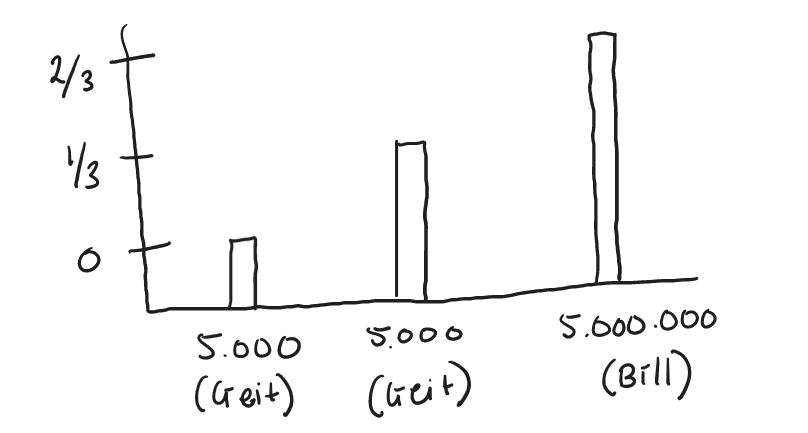
\includegraphics{graf.jpg}
\caption{Líkurnar á því að fá 5.000kr fyrir eina geit eru 0 þar sem
þátttastjórnandi opnar alltaf eina hurð með. Líkurnar á því að fá
5.000kr fyrir aðra geit eru 1/3}
\end{figure}

Til að skýra þrautina enn frekar var hermt eftir 100000 þátttökum í
leiknum og gróðinn reiknaður í hvert sinn sem ekki var skipt um hurð
eftir að þátttastjórnandi opnar eina hurð með geit.

\begin{Shaded}
\begin{Highlighting}[]
\NormalTok{hurd }\OtherTok{\textless{}{-}} \FunctionTok{c}\NormalTok{(}\StringTok{\textquotesingle{}bill\textquotesingle{}}\NormalTok{,}\StringTok{\textquotesingle{}geit\textquotesingle{}}\NormalTok{,}\StringTok{\textquotesingle{}geit\textquotesingle{}}\NormalTok{)}

\CommentTok{\#Spilari skiptir ekki}
\NormalTok{j }\OtherTok{\textless{}{-}} \DecValTok{0}
\NormalTok{win2 }\OtherTok{\textless{}{-}} \DecValTok{0}
\NormalTok{loss2 }\OtherTok{\textless{}{-}} \DecValTok{0}
\NormalTok{utkoma }\OtherTok{\textless{}{-}} \DecValTok{0}

\ControlFlowTok{for}\NormalTok{(j }\ControlFlowTok{in} \DecValTok{1}\SpecialCharTok{:}\DecValTok{100000}\NormalTok{)\{}
\NormalTok{  ValSpilara }\OtherTok{\textless{}{-}} \FunctionTok{sample}\NormalTok{(hurd,}\DecValTok{1}\NormalTok{)}
  
  \ControlFlowTok{if}\NormalTok{(ValSpilara}\SpecialCharTok{==}\StringTok{\textquotesingle{}bill\textquotesingle{}}\NormalTok{)\{}
\NormalTok{    utkoma }\OtherTok{\textless{}{-}}\NormalTok{ utkoma }\SpecialCharTok{+} \DecValTok{5000}
\NormalTok{    j}\SpecialCharTok{+}\DecValTok{1}
\NormalTok{    win2 }\OtherTok{\textless{}{-}}\NormalTok{ win2}\SpecialCharTok{+}\DecValTok{1}
\NormalTok{  \}}
  \ControlFlowTok{if}\NormalTok{(ValSpilara }\SpecialCharTok{==}\StringTok{\textquotesingle{}geit\textquotesingle{}}\NormalTok{)\{}
\NormalTok{    utkoma }\OtherTok{\textless{}{-}}\NormalTok{ utkoma }\SpecialCharTok{+} \DecValTok{5}
\NormalTok{    j}\SpecialCharTok{+}\DecValTok{1}
\NormalTok{    loss2 }\OtherTok{\textless{}{-}}\NormalTok{loss2}\SpecialCharTok{+}\DecValTok{1}
\NormalTok{  \}}
\NormalTok{  j }\OtherTok{\textless{}{-}}\NormalTok{ j}\SpecialCharTok{+}\DecValTok{1}
\NormalTok{\}}
\NormalTok{utkoma}
\end{Highlighting}
\end{Shaded}

\begin{verbatim}
## [1] 166683650
\end{verbatim}

\begin{Shaded}
\begin{Highlighting}[]
\NormalTok{win2}
\end{Highlighting}
\end{Shaded}

\begin{verbatim}
## [1] 33270
\end{verbatim}

\begin{Shaded}
\begin{Highlighting}[]
\NormalTok{loss2}
\end{Highlighting}
\end{Shaded}

\begin{verbatim}
## [1] 66730
\end{verbatim}

Hermt var einnig eftir 100000 þátttökum í leiknum og reiknaður gróðinn í
hvert sinn þegar þátttakandi skiptir um hurð eftir að þátttastjórnandi
hefur opnað eina hurð með geit

\begin{Shaded}
\begin{Highlighting}[]
\CommentTok{\#Spilari skiptir}
\NormalTok{hurd }\OtherTok{\textless{}{-}} \FunctionTok{c}\NormalTok{(}\StringTok{\textquotesingle{}bill\textquotesingle{}}\NormalTok{,}\StringTok{\textquotesingle{}geit\textquotesingle{}}\NormalTok{,}\StringTok{\textquotesingle{}geit\textquotesingle{}}\NormalTok{)}

\NormalTok{i }\OtherTok{\textless{}{-}} \DecValTok{0}
\NormalTok{win }\OtherTok{\textless{}{-}} \DecValTok{0}
\NormalTok{loss }\OtherTok{\textless{}{-}} \DecValTok{0}
\NormalTok{SkiptiUtkoma }\OtherTok{\textless{}{-}} \DecValTok{0}

\ControlFlowTok{for}\NormalTok{(i }\ControlFlowTok{in} \DecValTok{1}\SpecialCharTok{:}\DecValTok{100000}\NormalTok{)\{}
\NormalTok{  Spilari }\OtherTok{\textless{}{-}} \FunctionTok{sample}\NormalTok{(hurd,}\DecValTok{1}\NormalTok{)}
\NormalTok{  Monty }\OtherTok{\textless{}{-}} \FunctionTok{sample}\NormalTok{(hurd,}\DecValTok{1}\NormalTok{)}
  
  \ControlFlowTok{while}\NormalTok{ (Monty }\SpecialCharTok{!=} \StringTok{\textquotesingle{}geit\textquotesingle{}}\NormalTok{)\{}
\NormalTok{    Monty }\OtherTok{\textless{}{-}} \FunctionTok{sample}\NormalTok{(hurd,}\DecValTok{1}\NormalTok{)}
    \ControlFlowTok{if}\NormalTok{(Monty }\SpecialCharTok{==} \StringTok{\textquotesingle{}geit\textquotesingle{}}\NormalTok{)\{}
\NormalTok{      SpilariSkiptir }\OtherTok{\textless{}{-}} \FunctionTok{sample}\NormalTok{(hurd,}\DecValTok{1}\NormalTok{)}
\NormalTok{    \}}
\NormalTok{  \}}
  \ControlFlowTok{while}\NormalTok{(SpilariSkiptir }\SpecialCharTok{==}\NormalTok{ Spilari)\{}
\NormalTok{    SpilariSkiptir }\OtherTok{\textless{}{-}} \FunctionTok{sample}\NormalTok{(hurd,}\DecValTok{1}\NormalTok{)}
\NormalTok{  \}}
  \ControlFlowTok{if}\NormalTok{(SpilariSkiptir}\SpecialCharTok{==}\StringTok{\textquotesingle{}bill\textquotesingle{}}\NormalTok{)\{}
\NormalTok{    SkiptiUtkoma }\OtherTok{\textless{}{-}}\NormalTok{ SkiptiUtkoma }\SpecialCharTok{+} \DecValTok{5000}
\NormalTok{    win }\OtherTok{\textless{}{-}}\NormalTok{ win}\SpecialCharTok{+}\DecValTok{1}
\NormalTok{  \}}
  \ControlFlowTok{if}\NormalTok{(SpilariSkiptir}\SpecialCharTok{==}\StringTok{\textquotesingle{}geit\textquotesingle{}}\NormalTok{)\{}
\NormalTok{    SkiptiUtkoma }\OtherTok{\textless{}{-}}\NormalTok{ SkiptiUtkoma }\SpecialCharTok{+} \DecValTok{5}
\NormalTok{    loss }\OtherTok{\textless{}{-}}\NormalTok{ loss }\SpecialCharTok{+}\DecValTok{1}
\NormalTok{  \}}
\NormalTok{  i }\OtherTok{\textless{}{-}}\NormalTok{ i}\SpecialCharTok{+}\DecValTok{1}
\NormalTok{\}}
\NormalTok{SkiptiUtkoma}
\end{Highlighting}
\end{Shaded}

\begin{verbatim}
## [1] 333676490
\end{verbatim}

\begin{Shaded}
\begin{Highlighting}[]
\NormalTok{loss}
\end{Highlighting}
\end{Shaded}

\begin{verbatim}
## [1] 33298
\end{verbatim}

\begin{Shaded}
\begin{Highlighting}[]
\NormalTok{win}
\end{Highlighting}
\end{Shaded}

\begin{verbatim}
## [1] 66702
\end{verbatim}

Hér má sjá formúlu skilyrta líkindafallsins sem lýsir mögulegum útkomum
þegar búið er að opna eina hurð með geit bakvið. Mögulegu útkomurnar eru
fjórar. Ein útkoma er sí að þátttakandi vinni með því að halda sig við
upprunalega valið sitt, gefið að hann velji hurð A.

\[
P (Vinna | Skiptir Ekki) = P(A | A) * P(Vinna)
\] Önnur útkoma er sú að þátttakandi vinni ef hann skiptir um hurð,
gefið að hann velji hurð A. \[ 
P (Vinna | Skiptir ) = P(B eða C | A) * P(Vnna)
\] Þriðja útkoma er sú að þátttakandi tapi ef hann skiptir ekki um hurð,
gefið að hann velji hurð A. \[
P (Tapa | Skiptir Ekki ) = P(B eða C | A) * P(Tapa)
\] Fjórða útkoman er sú að þátttakandi tapi með því að skipta um hurð,
gefið að hann velji hurð A. \[
P(Tapa | Skiptir ) = P(A | B eða C ) * P (Tapa)
\]

Væntigildi gróðans í leiknum eru líkurnar á því að vinna bíl margfaldað
með verðmæti bílsins sem er svo samanlagt við líkurnar á því að vinna
geit margfaldað með verðmæti geitarinnar. Í þessu tilviki er verðmæti
bílsins fimm milljónir og verðmæti geitar er fimm þúsund krónur

Þegar þátttakandi skiptir ekki um hurð eftir að þátttastjórnandi hefur
opnað eina hurð með geit er væntigildi gróðans:

\[
E[X] = \frac{1}{3} * 5000000 + \frac{2}{3} * 5000
     = 1,669,999
\]

Væntigildi gróðans þegar einstaklingur skiptir um hurð eftir að
þátttastjórnandi opnar eina hurð með geit er: \[
E[X] = \frac{1}{3} * 5000 + \frac{2}{3} * 5,000,000
     = 3,334,999
\] Það má sjá að væntigildi gróðans er 3,334,999kr ef skipt er um hurð
þegar þátttastjórnandi hefur opnað eina hurð en væntigildi er
1,669,999kr ef ekki er skipt um hurð. Það er því hagstæðara að skipta um
hurð.

Til þess að það borgi sig að skipta um hurð í þessu tilviki þyrfti
verðmæti geitar að vera helmingur af verðmæti bílsins, eða 2,5 milljónir
króna.

Út frá þessum upplýsingum að ofan má draga þá ályktun að alltaf skuli
skipta um hurð í Monty Hall þrautinni.

\end{document}
